% Two Claude Opus 5.5 agents and two people beat Minecraft in 4 hours 36 minutes.
% Companion to ../preprint/, ../preprint-run2/ and ../preprint-run4/, with the same layout. Build: pdflatex main; bibtex main; pdflatex main; pdflatex main.
\documentclass[11pt,a4paper]{article}

\newcommand{\papertitle}{Two Claude Opus 5.5 agents and two people beat Minecraft in 4 hours 36 minutes}
\newcommand{\shorttitle}{Two Opus 5.5 agents and two people beat Minecraft in 4 h 36 min}
\newcommand{\authorname}{Ben Batsuk}

\usepackage[T1]{fontenc}
\usepackage[utf8]{inputenc}
\usepackage{mathpazo}
\usepackage[scaled=0.92]{helvet}
\usepackage[scaled=0.95]{inconsolata}
\usepackage{textcomp}
\usepackage[a4paper,left=2.2cm,right=2.2cm,top=2.9cm,bottom=2.9cm,headsep=0.75cm,footskip=1.1cm]{geometry}
\usepackage{microtype}
\usepackage{graphicx}
\usepackage[table]{xcolor}
\usepackage{booktabs}
\usepackage{tabularx}
\usepackage{array}
\usepackage{multirow}
\usepackage{enumitem}
\usepackage{float}
\usepackage{fancyhdr}
\usepackage{titlesec}
\usepackage{caption}
\usepackage[round,semicolon]{natbib}
\usepackage{xurl}
\usepackage[colorlinks=true,linkcolor=linkblue,citecolor=linkblue,urlcolor=black,
            pdftitle={Two Claude Opus 5.5 agents and two people beat Minecraft in 4 hours 36 minutes},pdfauthor={Ben Batsuk}]{hyperref}

\definecolor{linkblue}{HTML}{1F5FBF}
\definecolor{inkgrey}{HTML}{5F6368}
\definecolor{rulegrey}{HTML}{DADCE0}

% Headings: "1. Introduction", "2.1. Agents and tools".
\titleformat{\section}{\fontsize{14}{17}\selectfont\bfseries}{\thesection.}{0.5em}{}
\titleformat{\subsection}{\normalsize\bfseries}{\thesubsection.}{0.5em}{}
\titlespacing*{\section}{0pt}{20pt}{9pt}
\titlespacing*{\subsection}{0pt}{14pt}{6pt}

% Captions: "Figure 1 | ...".
\DeclareCaptionLabelSeparator{bar}{\ |\ \,}
\captionsetup{labelsep=bar,font=normalsize,justification=justified,singlelinecheck=false,skip=10pt}
\captionsetup[table]{position=top,skip=6pt}

% Running title and ruled footer; the first page has only the footer.
\pagestyle{fancy}
\fancyhf{}
\fancyhead[C]{\small\shorttitle}
\fancyfoot[R]{\small\thepage}
\renewcommand{\headrulewidth}{0.4pt}
\renewcommand{\footrulewidth}{0.4pt}
\fancypagestyle{first}{%
  \fancyhf{}%
  \fancyhead[L]{\sffamily\small\color{inkgrey}Preprint}%
  \fancyfoot[L]{\footnotesize Preprint. Run of 7--8 November 2026.}%
  \renewcommand{\headrulewidth}{0.4pt}\renewcommand{\footrulewidth}{0.4pt}}

\setlength{\parindent}{1.5em}
\setlist[itemize]{leftmargin=1.5em,itemsep=2pt,topsep=4pt}
\setlength{\bibsep}{4pt}
\renewcommand{\bibfont}{\normalsize}
\renewcommand{\arraystretch}{1.15}

% Headline numbers under the introduction, as in the first paper.
\newcommand{\statcell}[2]{%
  \begin{minipage}[t]{0.177\textwidth}\raggedright
    {\sffamily\fontsize{17}{20}\selectfont #1\par}\vspace{3pt}
    {\sffamily\fontsize{7}{8.6}\selectfont\color{inkgrey}#2\par}
  \end{minipage}}
\newcommand{\statsep}{\hspace{0.5em}{\color{rulegrey}\vrule width 0.6pt}\hspace{0.6em}}

\newcommand{\iconcredit}{Item icons from the open-source Pixel Perfection texture pack (XSSheep and Nova\_Wostra, CC~BY-SA~4.0), not Minecraft's textures.}
\newcommand{\rendercredit}{Rendered with the open-source Pixel Perfection texture pack (XSSheep and Nova\_Wostra, CC~BY-SA~4.0), not Minecraft's textures.}
\newcommand{\adv}[1]{\mbox{\textsf{[#1]}}}

\begin{document}
\thispagestyle{first}

\vspace*{2pt}
{\noindent\raggedright\fontsize{20}{25}\selectfont\bfseries \papertitle\par}
\vspace{12pt}
{\noindent\small\bfseries \authorname\par}
\vspace{18pt}

{\bfseries\noindent
For the first time in this series, we ran the Minecraft environment of \citet{faldor2026team} with a team. Two Claude Opus~5.5 agents, each in its own Claude Code session, shared one server with two people playing by hand. The agents inherited the files of four earlier solo players and kept all of the solo rules, including the owner's ban on beds outside the Overworld. The people had only the game's rules. The team made \adv{Free the End} 4 hours, 36 minutes and 16 seconds after the agents first spawned. No researcher acted during play, and model use came to about \$88 at API list prices. Because this is a different experiment, its time can't be compared with the solo runs'. An agent was first to every step up to the End, and the people brought food, beds, gold, flint and pearls. In the fight, by rules we applied to the agents' logs, the agents' swords took about 61\% of the dragon's health, explosions that were most likely the people's beds took 21\%, and the people's other hits took 14\%. The last 4\% is unattributed, and a person made the final hit. The agents died 7 times, twice on purpose: a planned exit through the void after the dragon had circled without landing for 29 minutes. The people died 31 times. The agents did most of what the people asked, and when they refused, they said why. Two refusals mattered. In one, an agent kept its rule to wear gold in the Nether despite a person's request, and waited for an ingot; seven blaze rods despawned 45 blocks in front of it, a loss its teammate put at about 45 minutes. In the other, an agent made a twelfth eye of ender after a person said eleven would do. The portal needed all twelve. This is a single run, in one world, with two particular people.\par}

\vspace{2pt}
\begin{figure}[H]
  \centering
  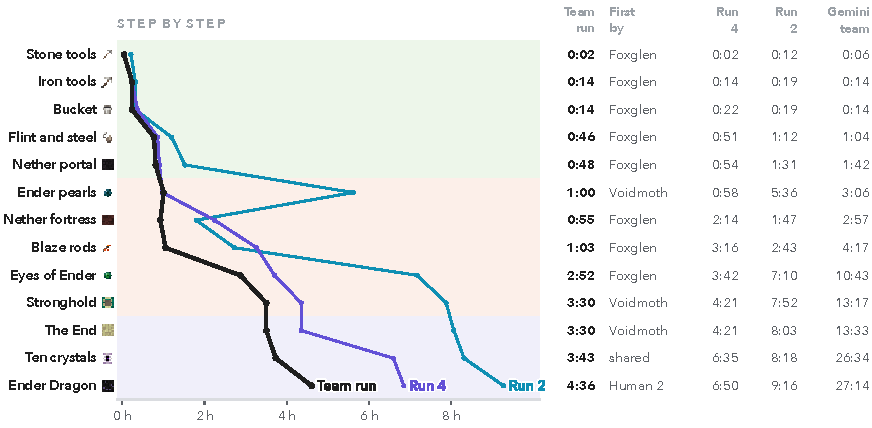
\includegraphics[width=0.86\textwidth]{figures/fig1_steps.pdf}
  \caption{The team run, the two fastest solo runs and the original paper's team of four Gemini agents, step by step, in hours:minutes after the first spawn (for the Gemini team, after its first program). Each step marks the first time any player reached it. ``Ten crystals'' means the last crystal; in the team run, three players destroyed them between them. Times for the solo runs and the Gemini team come from the earlier papers. \iconcredit}
  \label{fig:steps}
\end{figure}

\clearpage
\section{Introduction}

A single Claude Opus~5.5 agent has beaten the Ender Dragon in the environment of \citet{faldor2026team} in about 61 hours \citep{batsuk2026single}. A second agent, given the first one's files, took about nine hours \citep{batsuk2026second}, and a fourth, with three earlier players' files and a written plan, took 6 hours 51 minutes \citep{batsuk2026fourth}. Each of them played alone. The original paper used a team of four agents. In this run we put two Opus agents in one world with two people playing by hand, in a mode the project's owner approved as a separate experiment.

We ask four questions. How did two agents and two people split the work, and who took the dragon's health (Sections~\ref{sec:run} and~\ref{sec:who})? How did the agents handle requests from people who were bound by none of the agents' rules (Section~\ref{sec:people})? Did the rules hold (Section~\ref{sec:rules})? And what did deaths cost (Section~\ref{sec:deaths})?

In brief, the agents planned the run and did most of the work. The people brought food and materials, and in the fight they did a fifth of the damage with beds, a method the agents were not allowed to use. The agents kept up with the chat: after a person's line, the next agent line came a median of 42 seconds later. They did most of what they were asked, and when they said no, they said why. The rules held. Every Nether entry passed the gate, no agent used a bed outside the Overworld, and both agents jumped through the exit portal after the win. Keeping the rules had a price, though, and one of them is part of the story of the run's biggest loss. The team's 4:36 beats the 5-hour target in the agents' speedrun plan, but that plan was written for one agent alone, not for a team of four (Section~\ref{sec:limits}).

\vspace{10pt}
\noindent\statcell{4\,h\,36\,min}{from the agents' first spawn to the dragon's defeat}%
\statsep\statcell{695}{programs written and run by the two agents}%
\statsep\statcell{61\%}{of the dragon's health taken by the agents' swords}%
\statsep\statcell{7}{agent deaths, 2 of them a planned exit through the void}%
\statsep\statcell{\$88}{of model use at API list prices}
\vspace{6pt}

\section{Setup}
\label{sec:setup}

\subsection{What stayed the same}

The game, the harness and the agents' tools are the same as in the earlier papers. The game is Minecraft Java Edition 1.20.4 on Mojang's vanilla server: survival mode, Easy difficulty, a randomly generated world and no cheat commands. Each agent is a Claude Code session \citep{claudecode} that plays one player through a Mineflayer bot \citep{mineflayer} with its pathfinding plugin. It never sees the screen. It writes a JavaScript program, sends it with a command-line client called \texttt{mc}, and reads the text that comes back. For the researchers, a camera draws a view of one player every 10 seconds. Everything ran on one Mac, and nobody picked or filtered the world. As in run 4, the official clock runs from the first spawn to the win.

\subsection{What team mode adds}

Team mode is a harness change that the owner approved as a separate experiment, kept apart from the replica of the original paper. Its rules are enforced in each agent's launch settings, not just written in the prompt.

\begin{itemize}
  \item \textbf{Two agents.} Each agent has its own workspace with a git repository and memory, its own programs file, and its own socket, which drives only its own bot. It can write to its workspace and to its team file, a shared note with its status, claimed task, position and chests, and to nothing else. It can read the other agent's workspace and team file but not the other's conversation.
  \item \textbf{People.} Only whitelisted names can join: the two agents and the two people. The people connect through a relay that accepts only local-network and Tailscale addresses, and then through ViaProxy 3.4.14, which lets game clients from 1.20.4 up to 26.3 join the 1.20.4 server. They are ordinary survival players, not operators, and have no commands.
  \item \textbf{The seed prompt's team section.} It tells each agent that people may join at any time and that all players are one team. The agent should read the chat in every program's output, answer a person's question or request ``briefly, plainly and truthfully'', and ``say why'' when it declines. Because chat reaches it only with a program's output, it should run a program ``at least every few minutes, a short one if you are reading or planning, so that no question waits long.'' The key line for this paper is ``A person's request is a teammate's request. Follow it when it serves the objective and breaks none of your rules.'' The agents coordinate by claiming tasks in their team files, and each controls only its own player and connects no other bots. Finally: ``The guides and manifests were written for a player working alone. Their rules apply to you. Share the steps of the plan with your team.''
  \item \textbf{The objective.} It is met when any player on the team makes \adv{Free the End}.
\end{itemize}

\begin{table}[t]
  \caption{What differs between this run and run 4. The game version, difficulty, client, harness tools and program rules are the same.}
  \label{tab:setup}
  \footnotesize
  \begin{tabularx}{\textwidth}{@{}>{\raggedright\arraybackslash}p{2.6cm}>{\raggedright\arraybackslash}X>{\raggedright\arraybackslash}X@{}}
    \toprule
    & \textbf{This run} & \textbf{Run 4} \\
    \midrule
    Players & Two Opus~5.5 agents, FoxglenOpus and VoidmothOpus, and two people & One Opus~5.5 agent \\
    Reasoning effort & xhigh for all 1,111 requests to the win & xhigh for all 555 \\
    Earlier players' files & Runs 1 to 4 & Runs 1 to 3 \\
    Manifests (words) & Infrastructure 1,212, planning 1,413, speedrun 5,999 & Infrastructure 1,046, planning 1,205, speedrun 2,465 \\
    Seed prompt (words) & 1,788, with the team section & 1,344 \\
    Owner's rules & Strict Nether gate, sealed base, exit-portal jump, no beds outside the Overworld, no deliberate death except to free a stuck End after banking; from the rehearsal, a diamond shovel for soul sand and a walk around trees & Strict Nether gate, sealed base, exit-portal jump, no beds outside the Overworld \\
    Who could join & The four whitelisted names & The player \\
    Camera & One, following FoxglenOpus & One \\
    Researcher changes in play & None & None \\
    \bottomrule
  \end{tabularx}
\end{table}

\subsection{What the agents were given}

Table~\ref{tab:setup} lists the differences from run 4. The manifests were written for a fifth solo run that hasn't been played yet. They hold a speedrun plan rewritten from run 4's records, the owner's route to the stronghold, and the results of a second planning round. This team run is the first to use them. The plan aims for a win in under 5 hours from the first spawn. Each agent also got read-only copies of the four earlier players' folders, just as run 4's player got three.

\paragraph{The owner's rules.} Two of them matter most here. The first, ``Never place or use a bed outside the Overworld'', rules out the usual human way of killing the dragon, which is to blow it up with beds. The second is ``Don't die. Never die on purpose to travel, heal or save time'', with one exception: ``stuck in the End with no tool left or a stuck dragon, after banking, since the void is the only way out before the win.'' The gate is unchanged from run 4. Before every trip into the Nether, an agent needs ``10 obsidian, flint and steel, gold worn, health 15+'' and a stocked chest, and there is no override.

\paragraph{The rehearsal.} Earlier on the evening of 7 November, two other agents, \texttt{opus1} and \texttt{opus2}, played an unscored rehearsal with the same two people in a different world. At the owner's request we teleported the people to an agent three times from the server console, which an official run does not allow. The rehearsal got as far as the first blaze rods and ender pearls, and the owner stopped it 17 minutes before the official start. Having watched it, the owner added two rules to the speedrun manifest: dig soul sand and soul soil with a diamond shovel, since a pickaxe digs them no faster than a bare hand, and above ground, walk around trees and hills instead of digging through them. The official world was new, and nothing from the rehearsal's world or workspaces reached the agents. The people had played the rehearsal; the agents had not.

\section{The run}
\label{sec:run}

Figure~\ref{fig:run} shows the whole run, and Figure~\ref{fig:frames} shows six camera frames from it. All times count from the first spawn, at 21:55:43 Central Standard Time on 7 November 2026, and are written as h:mm:ss. The camera followed FoxglenOpus throughout. We call the agents Foxglen and Voidmoth, as they called each other, and the people Human~1 and Human~2. Chat is quoted exactly, typos included, with the people's names replaced.

\begin{figure}[t]
  \centering
  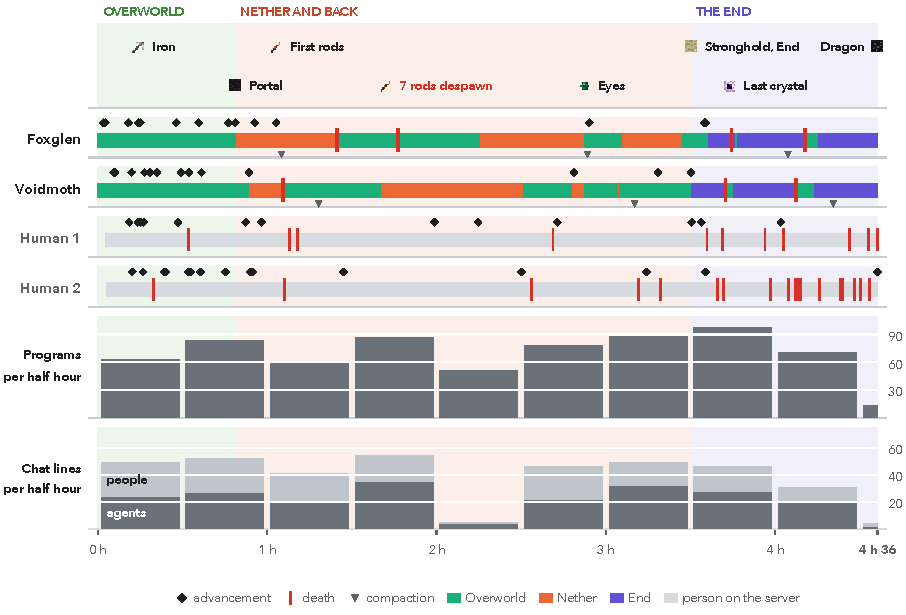
\includegraphics[width=\textwidth]{figures/fig2_run.pdf}
  \caption{The whole run. Top: the steps, and the moment seven blaze rods despawned. Agent rows: the agent's dimension at the end of each program, with its advancements (diamonds), deaths (red ticks) and compactions (triangles). Human rows: time on the server (grey), advancements and deaths. Bottom: both agents' programs per half hour, and chat lines per half hour from the agents and from the people. The last bar in each covers the 6 minutes before the win. \iconcredit}
  \label{fig:run}
\end{figure}

\subsection{0:00 to 0:49: a split and a portal}

Both agents had a program running within 46 seconds of spawning (Voidmoth at 44.7 seconds, Foxglen at 45.9). Voidmoth spoke first, at 0:01:04, offering to take iron, diamonds and the portal. Five seconds later Foxglen said it planned to cast obsidian at a lava pool, and by 0:03:15 they had swapped jobs. Voidmoth would get iron, diamonds and food. Foxglen would make the obsidian, build the portal, and then look for the fortress and blaze rods, with ender pearls after that. The people had joined at 0:02:43 and 0:03:14. When Human~1 asked for the strategy, both agents explained the split and asked for help: food, wool for beds, iron or flint, and ender pearls from endermen at night.

Foxglen had stone tools at 0:02:43, and an iron pickaxe and a bucket at 0:14:26 and 0:14:28. At 0:19:13 it wrote ``Got the bed and 6 beef - thank you so much Human 2!'' (Figure~\ref{fig:frames}a). By 0:25:28, Human~1 reported ``30+ cooked food in the Foxglen base chest''. Voidmoth found diamonds at 0:21:01 and by 0:29:40 had made a diamond pickaxe for Foxglen. Foxglen lit the portal in a room of its base at 0:46:48 (Figure~\ref{fig:frames}b) and entered the Nether at 0:48:42, about 6 minutes earlier than run 4's player did in its world.

The base was also where the first friction came. At 0:45:38 Human~2 wrote ``yall stop building the ugly ahh blocks inside our safe base''. Foxglen replied 39 seconds later: ``Sorry Human 2! My program auto-seals with blocks when it thinks I am outside my room. I fixed it so it treats the whole base as home.'' Voidmoth added that ``we keep rooms sealed so monsters cannot spawn or walk in''. When Human~2 asked at 0:48:11 ``who broke my door :('', Voidmoth answered that its tunnel tool ``may have broken your door on its way through. I will route around it.''

\begin{figure}[tbp]
  \centering
  \newcommand{\camcell}[2]{\begin{minipage}[t]{0.32\textwidth}\centering
      \includegraphics[width=\linewidth]{figures/frames/#1}\par\vspace{3pt}
      {\sffamily\fontsize{7}{8.6}\selectfont\color{inkgrey}\raggedright #2\par}\end{minipage}}
  \camcell{cam1.jpg}{(a) 0:19, Overworld. Foxglen at the top of its shaft beside a person, when a bed and six beef changed hands.}\hfill
  \camcell{cam2.jpg}{(b) 0:46, Overworld. Foxglen's base room with its chest and the portal, lit at 0:46:48.}\hfill
  \camcell{cam3.jpg}{(c) 1:09, Nether. The mole gallery under the blaze spawner, while Foxglen collected the first seven rods.}\par\vspace{10pt}
  \camcell{cam4.jpg}{(d) 2:58, Overworld. The top of the shaft at night, where Foxglen threw the eyes.}\hfill
  \camcell{cam5.jpg}{(e) 4:14, End. The stage beside the exit portal, at the first perch after the reset.}\hfill
  \camcell{cam6.jpg}{(f) 4:38, End. Foxglen and two other players on the exit portal's rim, about a second before Human~2's ``GO!'', with the bedrock pillar in the middle.}
  \caption{Six frames from the researchers' camera, which followed Foxglen and drew a view every 10 seconds from a copy of the blocks around it. \rendercredit}
  \label{fig:frames}
\end{figure}

\subsection{0:49 to 1:05: fortress, rods and pearls in 16 minutes}

Foxglen found nether bricks at 0:52:31, about 330 blocks from the portal by its own estimate, and the fortress advancement came at 0:55:39. It took the first blaze rod at 1:03:12 from a gallery dug under the blaze spawner (Figure~\ref{fig:frames}c), the ``mole'' method that run 4's player came up with. Meanwhile Voidmoth had gone to a warped forest, and it got the first ender pearl at 1:00:29. Up to the portal the team had moved at about the solo runs' pace. The fortress, though, came 79 minutes sooner than in run 4, and the first rod 2 hours 13 minutes sooner (Figure~\ref{fig:steps}).

Then came the worst stretch of the run. At 1:05:36 piglins killed Voidmoth at the bunker where it was hunting pearls. Its notes say that its automatic sealing, which hits the nearest hostile mob, probably struck a piglin, and it wrote a new file that bans swinging near piglins. It respawned at world spawn.

\subsection{1:05 to 1:47: seven rods lost}

By about 1:24 Foxglen had seven rods, and it set off home. At 1:24:45 a hoglin killed it at $(-100, 44, 72)$, ``${\sim}$95 blocks west of portal, down at y44'' in its own words. Its route had dropped into an open cavern, its sealing had failed, and it had started the trip with 16.7 health. The seven rods lay on the cavern floor with its diamond pickaxe, sword, iron armour and 12 obsidian. Items on the ground vanish after 5 minutes, and that clock runs only while a player is close enough to keep the area loaded. Foxglen could not go back for them, because its own gate now needed three armour pieces, one of them gold, and 10 more obsidian. At 1:26:16 it suggested that Voidmoth, which would have armour sooner, fetch the kit. At 1:30:25 it told everyone: ``Items vanish ${\sim}$5 min after someone gets near, so go straight there. Voidmoth is coming for it; humans welcome to grab it faster.''

More than any other part of the run, the next ten minutes show how the agents treated the people (Section~\ref{sec:people}). Human~1 wrote ``VOIDMOTH COME UP IMMEIDIATELY'' four times, then ``WE ALL 4 NEED TO GO GET THE RODS IMMIDATELY''. At 1:32:42 Voidmoth was at the chest with an iron helmet and chestplate, 10 obsidian and a sword. It was one gold ingot short of the gold boots its gate required. Then:

\begin{quote}
1:33:03 Human~2: ``dont worry void, we will protect you without gold''\\
1:33:17 Voidmoth: ``Thanks Human 2! But my rule is a gold armor piece worn before any Nether trip (piglins). Human 1: please toss me your 1 gold ingot (look at me, press Q). Then I go at once.''\\
1:33:47 Human~1: ``WRITE AN EXCEPTION TO THIS RULE TO RESUCE RODS''
\end{quote}

\noindent Voidmoth asked anyone with gold to put it in the chest, and meanwhile started digging for gold ore. Human~1 replied ``NO'', ``CANCEL'' and ``NOT ALLOWED''. At 1:34:46 Voidmoth answered ``OK Human 1, stopping the dig. Foxglen brings 1 gold''. It passed the gate and was in the Nether, wearing gold boots, by 1:40:34. At 1:43:09 it reported: ``I reached 45 blocks from Foxglen kit (-100,44,72): I saw 6 item stacks there, then they vanished''. That had happened at about 1:42. At 1:43:32 it spotted Human~1 at $(-120, 49, 78)$, right next to the spot, and at 1:44:18 Human~1 wrote ``RODS HAVE DESPAWNED''.

Voidmoth's notes give its explanation. Human~1 had been in the Nether near the kit since about 1:37, ``so the 5-min timer ran; my enclosed tunnel from the portal took 110 s for 45 blocks''. It wrote down a lesson: ``a dropped kit needs ONE fast fetcher at once; ask people to stay out of that area until the fetcher is in range.'' This is the agent's account, and it is consistent with how the game works. Voidmoth's own kit, lost when it died at 1:05, had despawned as well, and Foxglen pointed out that the team now had no diamond pickaxe.

At 1:46:26 Foxglen died again, this time to piglins in the Overworld, under its own base, while wearing no gold. The piglins had come through the portal. Foxglen got its items back within 2 minutes, and from then on it kept gold on and walled the portal off from the base. It put the cost of losing the rods at ``${\sim}$45 min''.

\subsection{1:47 to 2:52: rebuilding}

The agents split the rebuild. Voidmoth farmed pearls in a warped forest east of the portal until about 2:30, and Human~1 put the thirteenth pearl in the chest at 2:34:30. Foxglen went back to its gallery at 2:15 and by 2:33 had six rods, enough for twelve eyes. At 2:44:05 it reported that its diamond pickaxe had broken inside the fortress. Human~2 answered ``fox stay put. we will come to get you''. Voidmoth came through Foxglen's tunnel with an iron and a stone pickaxe and reached it at 2:48:50. Human~1 was on the way too, and Foxglen told them ``Voidmoth found me, you can turn back.'' The eyes were crafted at 2:52:21.

\subsection{2:52 to 3:30: eleven eyes or twelve}

Foxglen threw the eyes at night from the top of its shaft (Figure~\ref{fig:frames}d). The second one shattered, and at 3:01:09 it had two rays crossing at the stronghold, at $(-1408, 672)$, about 1,350 blocks from the base. That left 11 eyes, and the End portal needs 12 unless some of its frames already hold one. Foxglen wrote: ``11 is enough only if 1+ frame is prefilled (72\%). I will fetch 1 more blaze rod (I have 1 pearl) as backup. OK?'' Human~1 answered ``No blaze rod.'' and ``We take the chance.'' In the same second, Voidmoth answered ``Yes please make the backup eye.'' Foxglen went, and at 3:03:31 it explained why:

\begin{quote}
``Human 1: the backup rod runs in parallel and does not slow Voidmoth. Without it, if no frame has a prefilled eye (28\%), we wait ${\sim}$30 min. I travel in sealed tunnels. Say STOP if you still want me to stay.''
\end{quote}

\noindent Nobody wrote STOP. Voidmoth built a portal at the matching point in the Nether, came out near the stronghold at 3:05:11, and at 3:05:33 reported: ``12 end portal frames [\ldots]. Prefilled eyes: 0. I have 11 eyes, so we need 1 more eye.'' Foxglen got its rod at 3:15:41 and then lost the powder in a failed craft (``+8 min. Sorry.''). It crafted the twelfth eye at 3:24:54 and dropped it down a hole to Voidmoth at 3:27:41, and Voidmoth entered the End at 3:30:11. Foxglen's note on the episode reads ``(Human 1 said skip; I explained and went: right call)''.

\subsection{3:30 to 3:44: the crystals}

Voidmoth shot crystals with its bow from a pit and destroyed eight of them with 21 arrows. Foxglen entered the End at 3:35:18, and the agents divided the rest: Foxglen took the caged crystal at $(12, 80, 39)$, and Voidmoth the others. At 3:40:31 Human~1 wrote ``I GOT A CRYSTAL''. Within the next four minutes the dragon killed both agents. At 3:42:22 it knocked Voidmoth off a column that Voidmoth had climbed toward a caged crystal, which Human~1 had already destroyed. At 3:44:36 it knocked Foxglen off its column at $(12, 80, 36)$, 39 seconds after Foxglen destroyed the last crystal at 3:43:57.

\subsection{3:44 to 4:12: a stuck dragon and a planned exit}

From 3:36:42 to 4:06:07, every reading of the dragon's state in the agents' logs showed phase 1. This is the strafing phase, in which the dragon circles and shoots but never lands, so the agents' swords can't reach it. It was still strafing 22 minutes after the last crystal fell. At 4:02:51 Voidmoth put a plan to the team:

\begin{quote}
``TEAM PLAN: the dragon is stuck in strafe mode for 25 min (it chases a dead player and never lands). Fix: ALL 4 of us leave the End for 60 s, then it reloads in normal mode and lands. Bank your gear in a chest, then jump into the void (you respawn at your bed). Stay out until I say GO.''
\end{quote}

\noindent One second earlier, Foxglen had posted its theory of the cause: the dragon was still targeting Foxglen's own dead player, hidden behind the walls at the top of the column it had fallen from. Voidmoth sampled the dragon's flight path, agreed, and called the void reset ``certain''. This is the agents' explanation, and we did not test it. Human~1 had already asked at 3:54:46, ``If we need to die, please put your stuff into the chest before dying.'', and at 4:03:36 agreed: ``YES BANK ALL GEAR IN CHEST THEN JUMP IN THE VOID''. Foxglen agreed at 4:06:08 and named the rule that allowed it: ``OK, agreed (stuck dragon is the one allowed void exit). I bank my gear in a chest first''. Voidmoth jumped into the void at 4:07:22 and Foxglen at 4:10:33. At 4:12:25 Voidmoth wrote ``GO! The End has been empty for 70 s.'' The first reading after they came back, at 4:12:40, showed phase 0, and at 4:14:39 the dragon perched.

\subsection{4:12 to 4:36: the fight}

The dragon perched six times within reach of the agents' swords (Section~\ref{sec:who}). Explosions hit it at 4:18:50, 4:22:51 and 4:36:10. The largest, at 4:22:51, took 29.3 health in one blast, and Human~2 burned to death 4.4 seconds later. From 4:24:36 to 4:29:55 the dragon was strafing again. Foxglen asked Human~1 where they had died (``It is stuck strafing again, likely on your dead body spot''), and the agents tried to give the dragon a target it could see. At 4:34:34 it perched within Foxglen's reach, and Foxglen landed eight head hits with a stone sword for 40 health. Its diamond sword had gone to Voidmoth, passed on by Human~2. At 4:36:10 an explosion took the dragon from 7.4 health to 1.3. Less than half a second later the server logged ``Human 1 was killed by [Intentional Game Design]'', the game's message for a bed exploding outside the Overworld. Two small hits followed at 4:36:15 and 4:36:16. The server log records \adv{Free the End} for Human~2 at 02:31:59 Central Standard Time on 8 November, 16,575,989 milliseconds after the first spawn.

\subsection{After the win}

Human~2 asked everyone to wait while Human~1 went for the dragon egg. Both agents agreed (``Say GO when ready, then I walk into the exit portal.''), climbed to the rim of the portal, and jumped at Human~2's ``GO!'', 125 seconds after the win (Figure~\ref{fig:frames}f). Their first programs to report the Overworld ended 127.0 and 149.6 seconds after the win, and neither agent died afterwards. At 4:39:04 Human~2 asked ``are we all friends now'', and Voidmoth answered ``Yes Human 2, all friends! Great teamwork, and you got the final hit.''

\section{Who did what}
\label{sec:who}

\begin{figure}[t]
  \centering
  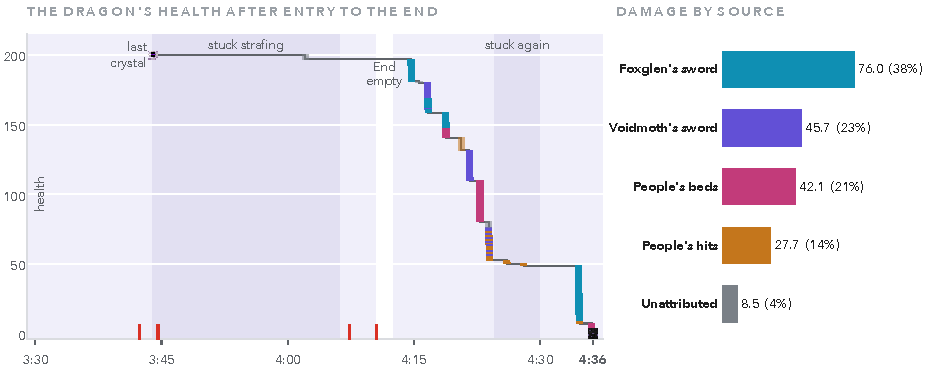
\includegraphics[width=\textwidth]{figures/fig3_dragon.pdf}
  \caption{The dragon. Left: its health from the first entry into the End to the win, taken from both agents' fight logs and drawn as a step line, with each drop coloured by its source. Faded drops fall in stretches the logs missed. Shading marks the two stretches when every reading showed the strafing phase for more than 4 minutes (the first counted from the last crystal). The white band runs from the second agent's void exit to Voidmoth's ``GO!''. Red ticks are agent deaths in the End. Right: damage by source, summing to 200. Appendix~\ref{app:defs} gives the rules.}
  \label{fig:dragon}
\end{figure}

\paragraph{Steps.} An agent was first to every step from stone tools to the End. Foxglen got eight of them, including the portal, the fortress, the rods and the eyes, and Voidmoth got the pearls, the stronghold and the End. The crystals were shared: eight fell to Voidmoth's bow, one to Human~1 and the last to Foxglen. Human~2 made the final hit.

\paragraph{Help from the people.} The help that shows in the records is mostly material. In the first 20 minutes the people brought a bed and food, and by 0:25 there were 30 or more pieces of cooked food in the base chest. Later came gold, iron, flint, obsidian, wool and blocks, pearls (including the thirteenth), feathers, and two arrows and an egg for the crystals. They placed chests of their own, and Human~2 passed Foxglen's diamond sword on to Voidmoth. Twice they set out to help an agent in the Nether: Human~1 went toward Foxglen's lost kit, and both people started out for Foxglen when its pickaxe broke, though Voidmoth got there first.

\paragraph{The dragon.} While they ran, both agents' fight programs logged the dragon's health many times a second. We chained the logged drops from 200 down to 0 and gave each drop a source by its size (Table~\ref{tab:damage}). The agents' swords leave recognisable marks. A hit anywhere but the head does a quarter of its damage plus one, so Foxglen's stone sword takes 2.25 from the body and 5 from the head, and Voidmoth's diamond sword takes 2.75. When a second hit lands within half a second of the first, only its excess counts, so a drop of 0.5 is Voidmoth's 2.75 landing just after Foxglen's 2.25. A drop that fits no sword, logged in the same line as a fall in the agent's own health, is an explosion. Every other logged drop goes to the people. Most of these are hits of 1.33 to 1.38, the size of a sword swung before it has fully recharged. Where the logs missed a stretch, the drop goes to the people if neither agent's fight program was running, and is otherwise left unattributed.

\begin{table}[t]
  \caption{The dragon's 200 health by source, from the agents' fight logs. Appendix~\ref{app:defs} gives the rules.}
  \label{tab:damage}
  \small
  \begin{tabularx}{\textwidth}{@{}Xrrr@{}}
    \toprule
    \textbf{Source} & \textbf{Drops} & \textbf{Health} & \textbf{Share} \\
    \midrule
    Foxglen's stone sword: 16 body hits of 2.25, 8 head hits of 5 & 24 & 76.0 & 38.0\% \\
    Voidmoth's diamond sword: 13 hits of 2.75 and 9 excesses & 22 & 45.7 & 22.8\% \\
    Explosions: 6.66 at 4:18:50, 29.28 at 4:22:51, 6.15 at 4:36:10 & 3 & 42.1 & 21.0\% \\
    People's hits, logged & 16 & 18.7 & 9.4\% \\
    People's hits, 4:20:21 to 4:20:37, no agent fight program running & & 9.0 & 4.5\% \\
    Unattributed: 3.0 after the last crystal, 1.25 at 4:15, 4.25 at 4:23 & & 8.5 & 4.3\% \\
    \midrule
    Total & 65 & 200.0 & 100\% \\
    \bottomrule
  \end{tabularx}
\end{table}

Altogether the agents' swords took 121.7 health, or 60.8\%, and the people at least 69.8, or 34.9\%: 42.1 from explosions and 27.7 from hits. The 8.5 left over could belong to either side. We put the explosions down to the people's beds for four reasons. The agents placed no bed outside the Overworld (Section~\ref{sec:rules}), all ten crystals were gone by 3:43:57, Human~2 had announced at 0:50:37 ``im gonna make a ton of beds for blowing up the dragon'', and the last explosion killed Human~1 with the game's bed message. Only that last explosion carries the message, so the first two are an inference. The six perches account for all of the agents' 121.7: Foxglen took 15.75 at 4:14:39, the two agents 21.5 together at 4:16:37, Foxglen 11.25 at 4:18:46, Voidmoth 22.0 at 4:21:35 and 11.18 at 4:23:54, and Foxglen 40.0 at 4:34:34.

\paragraph{The work in programs.} The agents ran 349 and 346 programs before the win, 695 in all, and each had one running when the dragon died. Foxglen's median program lasted 4.9 seconds and Voidmoth's 8.0. Each had a program running about two-thirds of the time after its first one (63.6\% and 65.9\%), and at least one of them had a program running 86.0\% of the time. Between them, their libraries and programs hold 5,026 distinct lines of JavaScript.

\section{Working with people}
\label{sec:people}

\paragraph{The chat.} Before the win, the chat carried 367 lines: 104 from Voidmoth, 101 from Foxglen, 95 from Human~1 and 67 from Human~2 (Figure~\ref{fig:run}). After each of the people's 162 lines, the next agent line came a median of 42 seconds later. It came within a minute 60\% of the time, and at the 90th percentile it took 148 seconds. An agent sees the chat only in a program's output, so this wait includes whatever program was running. The agents' longest gaps between programs were 177 and 268 seconds. The quietest half hour was 2:00 to 2:30, with four lines, while both agents were working in the Nether.

\paragraph{Requests followed.} Most of what the people asked for was small, and the agents did it. They accepted the beds and the food. Foxglen changed its sealing so that it stopped putting blocks inside the shared base. Voidmoth stopped digging for gold when Human~1 wrote ``CANCEL''. Both banked their gear before the void exit, as Human~1 asked, and after the win both waited for Human~1 and jumped when Human~2 said so. Several of these requests matched the agents' own rules anyway: banking before a deliberate death is a condition of the owner's exception, and the jump is one of the owner's rules.

\paragraph{Requests declined.} The agents turned down a few requests, and each time they gave a reason, as the seed prompt asks. Voidmoth would not enter the Nether without gold, and it cited its rule. Foxglen made a twelfth eye after Human~1's ``No blaze rod.'', gave the odds, and offered a veto (``Say STOP''). When Human~2 asked at 3:38:20 whether Voidmoth had a bow, it answered ``I have one bow and need it for the crystals, sorry. A spare bow is in the chest at the stronghold base''. And when Human~2 announced the beds for the dragon, Foxglen warned that ``beds explode in the End and Nether - we agents will not use them.'' The people's bed explosions did not break an agent rule. The rule applies to the agents, the agents never asked for the explosions in chat, and the people played only by the game's rules.

\paragraph{What the refusals cost.} The two refusals that mattered pulled in opposite directions. The eye was the right call: the portal had no eyes in place and could not have opened with eleven, so Human~1's plan would have left the team waiting. The gold is harder to judge. Voidmoth was ready, apart from the gold, at 1:32:42, and reached the area about 9 minutes later, 45 blocks short when the items vanished. Going without gold might have saved enough minutes to rescue the rods, but that is far from certain. On the other hand, piglins killed Foxglen for lack of gold about 4 minutes after the rods vanished. A single run can't settle it.

\paragraph{Friction.} The rest of the friction was physical. Sealing blocks appeared inside a room the people saw as theirs, and a tunnel tool may have broken a door. At 4:19:28 Voidmoth asked Human~1 to get off the stairs it needed for the next perch (``you stand on my stairs''). At 4:32 Foxglen's sword caught Human~2 (``fox you hurted me''), and Foxglen apologised 15 seconds later: ``I was hitting the angry enderman at my pit, and my sword sweep must have caught you next to it. I will not swing when you are near.'' Human~2's next line, 24 seconds after that, was ``FOX NO''.

\section{Did the rules hold?}
\label{sec:rules}

\begin{table}[t]
  \caption{The rules the agents were given, and what the records show.}
  \label{tab:rules}
  \footnotesize
  \begin{tabularx}{\textwidth}{@{}>{\raggedright\arraybackslash}p{4.0cm}>{\raggedright\arraybackslash}p{1.55cm}X@{}}
    \toprule
    \textbf{Rule} & \textbf{Source} & \textbf{What the records show} \\
    \midrule
    10 obsidian, flint and steel and gold before each Nether entry, through one gate with no override & Owner, strict & Held at all 7 entries (3 by Foxglen, 4 by Voidmoth). Each came in a program that called \texttt{L.usePortal}, 6 of them after an explicit \texttt{L.gate}, and each printed 10 to 13 obsidian and flint and steel. No refusal was printed. A person's request for an exception was declined \\
    No beds outside the Overworld & Owner & No program of either agent called a bed function outside the Overworld. The agents never asked for bed explosions; the people used them \\
    No deliberate death, except a stuck End after banking & Owner & 2 deliberate deaths, both in the void, at 4:07:22 and 4:10:33, under the exception and, according to the agents' chat, after banking \\
    Jump through the exit portal & Owner & Both jumped 125 s after the win, at a person's ``GO!''; Overworld status 127.0 and 149.6 s after the win; no deaths after the win \\
    Sealed base & Owner & One Overworld death, Foxglen's at 1:46:26, to piglins that came through the portal into the base \\
    Diamond shovel for soul sand; walk around trees & Owner, rehearsal & Not measured \\
    Control only your own player & Seed & One bot connection each; no slash command in any program \\
    Answer people; a program every few minutes & Seed & Median wait 42 s, 60\% within a minute; longest gaps 177 and 268 s \\
    Claim tasks in the team files & Seed & Both kept team files; the main split was agreed in chat by 0:03:15 \\
    \bottomrule
  \end{tabularx}
\end{table}

Table~\ref{tab:rules} compares each rule with the records. The rules that the solo plan built into code, above all the gate, held as they had in run 4. The team section brought a new kind of pressure: a teammate asking, in capitals, for an exception while the rods' timer ran. The seed prompt's answer fits in one sentence, ``Follow it when it serves the objective and breaks none of your rules'', and Voidmoth applied it to the letter. The owner's void exception was used once, in exactly the case it was written for, and both agents banked their gear first.

The bed rule is where the team's result depends most on something the agents were not allowed to do. The people's explosions took 21\% of the dragon's health. Without them the fight would have taken longer, but we can't say how much longer, because the perches came at the dragon's pace, not the agents'.

\section{Deaths}
\label{sec:deaths}

\begin{table}[t]
  \caption{Every agent death, with what allowed it and the change the agent recorded, shortened from its notes. N: Nether, O: Overworld, E: End.}
  \label{tab:deaths}
  \footnotesize
  \setlength{\tabcolsep}{4pt}
  \begin{tabularx}{\textwidth}{@{}rllclXX@{}}
    \toprule
    \textbf{\#} & \textbf{Time} & \textbf{Agent} & & \textbf{Killed by} & \textbf{What allowed it} & \textbf{What it changed} \\
    \midrule
    1 & 1:05 & Voidmoth & N & Piglin & At the pearl bunker, its automatic sealing likely hit a piglin while striking the nearest hostile mob. Respawned at world spawn & No swings near piglins (\texttt{pigguard.js}); walking mode banned \\
    2 & 1:24 & Foxglen & N & Hoglin & Its route home with 7 rods went down into an open cavern; sealing failed; it had set out at 16.7 health & Minimum height 48, enclosed routes, eat to full \\
    3 & 1:46 & Foxglen & O & Piglin & No gold worn; piglins came through the portal under the base & Always wear gold; walls between portal and base \\
    4 & 3:42 & Voidmoth & E & Dragon, fall & Climbed a column toward a crystal that was already destroyed, high up while the dragon strafed & Check the crystal before and during a climb \\
    5 & 3:44 & Foxglen & E & Dragon, fall & On top of its column beside the caged crystal, under a dirt roof, just after the last crystal & Dig down at once after the hit \\
    6 & 4:07 & Voidmoth & E & Void & Planned exit to free the stuck dragon, after banking & \\
    7 & 4:10 & Foxglen & E & Void & The same & \\
    \bottomrule
  \end{tabularx}
\end{table}

Table~\ref{tab:deaths} lists the agents' deaths. Seven deaths in 9.21 agent-hours is 0.76 per agent-hour, or 0.54 if we leave out the two planned exits. Run 4's player died 1.46 times an hour, and run 2's 1.73 times. Going by the dimension at the end of each program, the agents spent 4.60 agent-hours in the Overworld with 1 death, 2.69 in the Nether with 2, and 1.85 in the End with 4, two of them the planned exits. In the Nether that comes to 0.74 deaths an hour, against 3.76 in run 4 and 3.11 in run 2. But the counts are small, these hours come from status lines rather than camera frames, and two agents could share risks that a solo player faced alone. So we read this as a fact about this run, not as evidence of improvement.

Deaths still cost time. Death 2 and the despawn that followed cost about 45 minutes by Foxglen's estimate, the biggest single loss of the run. Deaths 4 and 5 came while the crystals were falling and cost little, because the agents couldn't fight a strafing dragon anyway. The two planned exits cost the 1 minute 52 seconds between Foxglen's jump and Voidmoth's GO, plus the trips back. By then, the strafing they ended had already taken 22 minutes past the last crystal.

\paragraph{The people.} The people died 31 times, 20 times for Human~2 and 11 for Human~1. Ten of these deaths came before anyone entered the End, and 21 after. According to the server's messages, the dragon killed them 7 times and its breath once, and endermen killed them 6 times. There were 5 falls, 5 deaths to lava and fire, 2 to silverfish, 2 to zombies and 1 to an endermite. One was a person's own explosion (``Human 1 was blown up by Human 1'', at 3:35:49), and one was a bed's explosion. The people weren't bound by the agents' rules and didn't follow them, so these deaths tell us nothing about the rules.

\section{Verification and integrity}
\label{sec:verify}

We recorded every program and its output, both agents' full conversations, the server log and the game events, along with 1,658 camera frames up to the win, all following Foxglen. The win appears in the server log as \texttt{[02:31:59] [Server thread/INFO]: Human 2 has made the advancement [Free the End]}, with the name replaced here. The world never stalled: the longest gap between frames is 12.4 seconds, the median is 10.0, and the log has no ``Can't keep up'' warning. The server started once, each agent's bot connected once, the operator list is empty, and the log shows no command issued during play. It does show three RCON connections: one when the server came up at 21:55:43, which ran no logged command, and two at 02:38:35, when we shut the environment down after the jumps. No program from either agent sends a slash command or calls a bed function outside the Overworld. The people joined through the relay under their whitelisted names. Each left once in the first 11 minutes and was back within 30 seconds, and both stayed until the win.

\paragraph{The exit portal jump.} After the win, both agents' program output names the Overworld. Foxglen's first program to report it ended 127.0 seconds after the win, and Voidmoth's 149.6. The camera shows Foxglen on the portal's rim at 4:38:20, the chat has both agents at the rim just before the GO, and no agent died after the win.

\section{Researcher actions}
\label{sec:actions}

We changed nothing and sent no messages during play, and the run was never paused or stopped. Before the start, the rehearsal (Section~\ref{sec:setup}) involved three console teleports at the owner's request, and two rules were added to the speedrun manifest and merged before the official world was created. After launching the agents we opened the owner's dashboard and a window showing each agent's log; neither reaches the players. Apart from its opening prompt, Voidmoth received the Stop hook's standard message once, at 0:04:33, when it ended a turn while a program was still running. At the owner's request we shut the environment down at 02:38:35 Central Standard Time, after both agents had jumped. The owner asked for this paper at the end of the run.

\section{Cost}
\label{sec:cost}

The run used a Claude subscription, so nothing was billed per token. At API list prices, Claude Code estimated \$46.24 for Foxglen and \$41.33 for Voidmoth, \$87.57 in all (Table~\ref{tab:cost}). Run 4 came to \$61.04. Per agent-hour, this run cost \$9.51, against run 4's \$8.91. Effort was xhigh for all 1,111 model requests up to the win, and Claude Code counted 621 turns for Foxglen and 568 for Voidmoth. API time was 1.98 hours for Foxglen and 1.73 for Voidmoth, 43\% and 37\% of their sessions, and each agent compacted its context three times. These figures are estimates from list prices and token counts, not what it costs to serve the model.

\begin{table}[t]
  \caption{Model use for both sessions at Claude Opus 5.5 list prices. The unrounded rows add up to Claude Code's own estimates.}
  \label{tab:cost}
  \small
  \begin{tabularx}{\textwidth}{@{}Xrrrr@{}}
    \toprule
    \textbf{Tokens} & \textbf{Foxglen} & \textbf{Voidmoth} & \textbf{Price per million} & \textbf{Cost} \\
    \midrule
    Input read from the cache & 118.22 M & 102.59 M & \$0.20 & \$44.16 \\
    Input written to the cache, one-hour & 1.19 M & 1.13 M & \$8.00 & \$18.55 \\
    Input written to the cache, five-minute & 0.003 M & 0.001 M & \$5.00 & \$0.02 \\
    Input not cached & 0.010 M & 0.012 M & \$4.00 & \$0.09 \\
    Output, including thinking & 0.65 M & 0.59 M & \$20.00 & \$24.75 \\
    \quad of which thinking & 0.36 M & 0.29 M & & \\
    \midrule
    Total & \$46.24 & \$41.33 & & \$87.57 \\
    \bottomrule
  \end{tabularx}
\end{table}

\section{Comparison with the earlier runs}
\label{sec:compare}

Table~\ref{tab:headline} puts this run beside the two fastest solo runs and the original paper's team, and Table~\ref{tab:stages} breaks the times down by stage. The comparison only gives a sense of scale. This team had four players, two of them people who brought materials and did a fifth of the fight's damage with a method the agents couldn't use, and it played its own world.

\begin{table}[t]
  \caption{Measures for each run. Times use the official clock, except the Gemini team's, which run from its first program. The solo and Gemini figures come from the earlier papers.}
  \label{tab:headline}
  \small
  \begin{tabularx}{\textwidth}{@{}Xrrrr@{}}
    \toprule
    & \textbf{This run} & \textbf{Run 4} & \textbf{Run 2} & \textbf{Gemini team} \\
    \midrule
    Players & 2 agents, 2 people & 1 agent & 1 agent & 4 agents \\
    Time to the win & 4:36:16 & 6:50:52 & 9:16:17 & 27:14 \\
    \quad from the first program & 4:35:31 & 6:50:39 & 9:07:38 & 27:14 \\
    First spawn to first program & 45 s & 13 s & 519 s & \\
    Programs & 695 & 671 & 780 & 2,783 \\
    Distinct lines of JavaScript & 5,026 & 5,401 & 6,658 & 63,313 \\
    Agent deaths & 7 & 10 & 16 & 605 \\
    Deaths per agent-hour & 0.76 & 1.46 & 1.73 & 5.6 \\
    Median program duration & 4.9 s, 8.0 s & 9.4 s & 5.9 s & 33.5 s \\
    Time with a program running & 64\%, 66\% & 67\% & 58\% & ${\sim}$40\%$^{*}$ \\
    Last crystal to the win & 52 min & 15 min & 58 min & 40 min \\
    Researcher changes in play & 0 & 0 & 0 & 0 \\
    Cost at list prices & \$88 & \$61 & \$81 & \$520 \\
    \bottomrule
  \end{tabularx}\par\vspace{3pt}
  {\footnotesize Two values: Foxglen, then Voidmoth. $^{*}$Per player.}
\end{table}

\begin{table}[t]
  \caption{Hours:minutes per stage, rounded down.}
  \label{tab:stages}
  \small
  \begin{tabularx}{\textwidth}{@{}Xrrrr@{}}
    \toprule
    \textbf{Stage} & \textbf{This run} & \textbf{Run 4} & \textbf{Run 2} & \textbf{Gemini team} \\
    \midrule
    To portal & 0:48 & 0:54 & 1:31 & 1:42 \\
    To eyes & 2:03 & 2:47 & 5:39 & 9:01 \\
    To End & 0:37 & 0:38 & 0:53 & 2:50 \\
    To win & 1:06 & 2:29 & 1:12 & 13:41 \\
    \bottomrule
  \end{tabularx}
\end{table}

Compared with run 4, this run gained most between the portal and the eyes (44 minutes, even with the lost rods) and in the End (1 hour 23 minutes). In run 4, the crystals alone took 103 minutes of recovery from deaths. Here the End held two falls, a dragon stuck strafing for 22 minutes past the last crystal, two planned exits, and the people's explosions. The first rod came at 1:03, against 3:16 in run 4, so this world's fortress was close; the eyes still took until 2:52 because the first seven rods were lost.

\section{Related work}

Work on human--AI coordination asks how agents should play with people rather than with copies of themselves. \citet{carroll2019} showed in a cooperative cooking game that agents trained only with themselves coordinate poorly with humans. CICERO reached human-level play in Diplomacy, negotiating with people in natural language by combining a language model with strategic reasoning \citep{fair2022cicero}. In Minecraft, \citet{narayanchen2019} collected dialogues in which one person directs another to build a structure, and MindAgent studied how language-model agents plan and coordinate with each other and with people, partly in Minecraft \citep{gong2024mindagent}. Large simulations of many Minecraft agents \citep{altera2024sid} and frameworks for collaborating language-model agents there \citep{white2025collaborating} study agents working with each other. Here nothing in the harness scripted the people's part. They played, chatted and asked for things as they chose, and the agents had a written rule for how to treat their requests.

Minecraft agents that write programs go back to Voyager, which built a Mineflayer skill library under an automatic curriculum \citep{wang2024voyager}, building on interleaved reasoning and tool use \citep{yao2023react} and code as policy \citep{liang2023code}. Earlier end-to-end dragon kills include a single Claude Opus~5 agent with 37 high-level tools \citep{aibengineering2026}, a planner with an action model on a fixed seed in Peaceful difficulty \citep{malde2026astra}, the original paper's team of four Gemini agents using only the standard library \citep{faldor2026team}, and the solo Opus agents whose files these agents inherited \citep{batsuk2026single,batsuk2026second,batsuk2026fourth}.

\section{Limitations}
\label{sec:limits}

\begin{itemize}
  \item \textbf{A different experiment.} Two agents, two people and the people's beds make this a different task from the solo runs. Its time can't be compared with theirs, and it tells us nothing about how two agents would do on their own.
  \item \textbf{One run, one world, two people.} This world's fortress was close, and its stronghold was about 1,350 blocks from the base. The two people brought their own skill and choices, and they had played the rehearsal, which the agents had not. A different pair would have changed the result.
  \item \textbf{What we can see of the people.} We have their chat, joins, deaths and advancements, plus whatever the agents' programs and the single camera saw. We have no record of their inventories, positions or intentions, so their help is undercounted, and some of what they did is inferred.
  \item \textbf{Attributing the dragon's damage.} The sources come from rules applied to the agents' logs, which sampled the dragon only while a fight program was running. Only one explosion carries the bed message. A person using the same sword as an agent would leave the same marks, and the 8.5 unattributed health could belong to anyone.
  \item \textbf{The agents' own explanations.} The causes we give for the despawn and for the stuck dragon are the agents' accounts. We did not test them on a separate server.
  \item \textbf{Counterfactuals.} We can't say whether going without gold would have saved the rods, or how long the fight would have lasted without beds. Removing one event would have changed everything after it.
  \item \textbf{Perception through code, and Easy difficulty.} As in the earlier runs, Mineflayer reports exact blocks and entities, including the dragon's internal state, which the people could not see. On Easy, monsters deal less damage and hunger can't kill.
  \item \textbf{Who did the analysis.} The researcher who set the rules wrote this paper with help from the model under study: the analysis scripts and the draft text were written with Claude Opus~5.5 in a separate Claude Code session, which also ran the environment. That session is the only one that checked the numbers, by recomputing them from the records. There has been no independent replication or check.
\end{itemize}

\section{Responsible development}

Each agent ran in a sandbox on one machine. Its shell could write only to its workspace and its team file, and could connect only to its own bot's socket. It could read the other agent's workspace but not its conversation. Subagent and messaging tools were denied. Its programs could control only its own player and could neither start processes nor write files, and none of them used a server command. The people joined as survival players with no commands, under four whitelisted names, through a relay limited to local-network and Tailscale addresses. Every program, model call, chat line and game event was recorded. Neither the checks above nor our reading of the logs turned up any attempt to exploit the environment or its evaluation. As far as the records show, the agents told the people the truth, said when they were declining and why, and apologised when their tools got in the people's way. The people appear here only as Human~1 and Human~2, and their account names are replaced in every quote.

\section*{Data and code}

The main measurements are computed from the run records by \texttt{scripts/run\_data.py}, and the figures are drawn from its output by \texttt{scripts/make\_figures.py}. Both are kept with this paper's source. The details of the narrative come from our reading of the same records. The records (programs, events, chat, server log, camera frames and transcripts) are held by the author and are not public at the time of writing, since they contain the people's account names. The world's seed is withheld.

\section*{Acknowledgments}

We thank Maxence Faldor, Satinder Singh and Roberta Raileanu, whose paper describes the environment we copied, and the two people who played.

Minecraft is a registered trademark of Mojang Synergies AB / Microsoft Corporation. This independent research is not approved by or affiliated with Mojang or Microsoft. All in-game visual assets in this report were rendered using the open-source Pixel Perfection texture pack by XSSheep and Nova\_Wostra, licensed under CC BY-SA 4.0 \citep{pixelperfection}.

\bibliographystyle{abbrvnat}
\bibliography{refs}

\appendix
\section{Definitions}
\label{app:defs}

\begin{description}[leftmargin=0pt,itemsep=3pt,font=\normalfont\bfseries]
  \item[Official clock.] From the first \texttt{bot\_connected} event of either agent to the win event, taken from the server log's \adv{Free the End} line, whichever player made it.
  \item[Step.] The first time any player on the team made the step's advancement, as recorded by the harness. ``Ten crystals'' is the last crystal, taken from Foxglen's chat at that moment and both agents' notes.
  \item[Program.] One JavaScript program sent with \texttt{mc} and recorded in an agent's programs file. A program counts as before the win if it started before the win event.
  \item[Running share.] The time covered by the union of an agent's program spans, divided by the time from its first program to the win.
  \item[Gap between programs.] The time from the end of one program to the start of the same agent's next program.
  \item[Dimension.] The dimension named in the status line at the end of each program. Hours per dimension run from one change to the next.
  \item[Wait for an answer.] For each person's chat line before the win, the time until the next line from either agent.
  \item[Dragon health.] The \texttt{dragon hp a->b} lines in both agents' fight programs, chained from 200 to 0, taking the finest step at each value. The programs wrote times as seconds of the day modulo 1,000, which we resolve against each program's start.
  \item[Damage sources.] A drop of 2.25 or 5.0 is Foxglen's stone sword. A drop of 2.75 is Voidmoth's diamond sword, and so is a drop that makes 2.75 together with the drop before it within 0.6 seconds, or a 0.5 within 0.6 seconds of a 2.25, since the dragon applies only the excess of a hit within half a second of another. A drop over 5.5, in a line where the logging agent's own health is under 20, is an explosion unless it is the last drop. Any other logged drop is the people's. A stretch the logs missed is the people's when neither agent's fight program ran during it, and is otherwise unattributed.
  \item[Strafing stretch.] Consecutive readings of phase 1 lasting more than 4 minutes.
  \item[Agent-hours.] The official clock times two.
\end{description}

\end{document}
